% !TEX root = diz.tex
Recently, an interdisciplinary research between the fields of Computer Science and Biology has been rapidly growing. Natural computing consists of three classes of methods:
\begin{itemize}
  \item Those that are based on the use of computers to simulate natural phenomena (Section~\ref{sec:bioinformatics}).
  \item Those that employ natural materials (e.g., molecules) to compute (Section~\ref{sec:biomolecular_computing}).
  \item Those that take inspiration from nature for the development of novel problem-solving techniques (Section~\ref{sec:biologically_inspired_computing_models}).
\end{itemize}

% Bioinformatics (slaves of biologists)

\section{Bioinformatics} % (fold)
\label{sec:bioinformatics}

Bioinformatics has undergone a fast evolving process, especially the areas of genomics and proteomics. Bioinformatics can be seen as the application of computing tools and techniques for the management of biological data. Just to mention a few:
\begin{itemize} 
  \item the design of efficient algorithms for DNA sequence alignment,
  \item the investigation of methods for prediction of the three-dimensional structure of molecules and proteins,
  \item the development of data structures to effectively store huge amount of structured data.
\end{itemize}

% section bioinformatics (end)

\section{Biomolecular computing} % (fold)
\label{sec:biomolecular_computing}

Biomolecular computing make use of molecules such as DNA and proteins to perform computations involving storing, retrieving and processing data. It takes advantage of the many different molecules to try many different possibilities at one, so it is somewhat similar to parallel computing.

Adleman in his 1994 report \cite{Adleman1994MolecularComputation} demonstrated a proof of concept use of DNA as a form of computation which solved the Hamiltonian path problem. Since then, various Turing machines have been proven to be constructible with DNA \cite{Kari2000DNAPCP}. 

DNA can also be used as a digital data storage with 5.5 petabits per cubic millimeter of DNA (see \cite{Church2012DNAStorage}). The information retrieval is, however, a slow process, as the DNA needs to be sequenced in order to retrieve data, so this method is intended mainly for a long-term archival of large amounts of scientific data.

% section biomolecular_computing (end)

\section{Biologically inspired computing models} % (fold)
\label{sec:biologically_inspired_computing_models}

On the other hand, the birth of biologically inspired frameworks started the investigation of mathematical models and their properties and technological requirements for their implementation by biological hardware.
Those frameworks are inspired by the nature in the way it ``computes'', and has gone through the evolution for billions of years.

Neural networks, genetic algorithms and DNA computing are already well established research fields.

\subsection{Neural networks} % (fold)
\label{sub:neural_networks}

Inspired by the human brain, which contains on average 86 billions neurons \cite{Azevedo09NumberOfNeurons}, neurophysiologist Warren McCulloch in 1943 proposed a mathematical model of artificial \index{Neural network} neural network.

A single perceptron computes a function $f(x)$, where $x$ is an input - a vector of real values.

The perceptron can learn itself by modifying parameters used to compute the function. This learning can be performed in various ways, we will mention only the supervised learning. Imagine a function with
\begin{itemize}
  \item input: perceptron's parameters
  \item output: error of the computed result $f(x)$
\end{itemize}
If the perceptron receives a feedback in form of error (from the supervision, e.g. dataset used to train the perceptron), it can modify its parameters such the error will be minimized in the future. This can be done through the gradient descent method, which is used to find a local minimum of a function.

A single perceptron can only compute linear functions, so they are often connected with other perceptron to form a neural network. Often it is practically unusable to say what is the purpose of a single neuron in a more complex neural networks.

Neural networks have broad applicability to real world problems and are best if the modeled system has some tolerance to error such as:
\begin{itemize}
  \item Image recognition: OCR, web search by image
  \item Music recognition by voice sample
  \item Speech recognition
  \item Time series forecast: weather, stock
  \item Diagnosing of illnesses
  \item Natural language processing
\end{itemize}

Besides real world problems, Graves et al. \cite{Graves14NeuralTM} extended the capabilities of neural networks by coupling them to external memory resources, allowing them to infer simple algorithms such as copying and sorting.

% subsection neural_networks (end)

\subsection{Evolutionary algorithms} % (fold)
\label{sub:evolutionary_algorithms}

\index{Evolutionary algorithms} Evolutionary algorithms are inspired by Darwin's theory of evolution. Basically, an algorithm starts with a population of random individuals (solutions to the problem). In each generation, the fitness of every individual is evaluated and the more fit individuals are replicated and mutated to form a new generation. The less fit individuals die.

Idea of evolutionary computing was introduced in the 1960's by I. Rechenberg. Nowadays they have been applied to find solution of many optimization problems. They also can be used to design or to train a neural network \cite{Montana:1989:TrainNeuronByGenetic}.

% subsection evolutionary_algorithms (end)

\subsection{L systems} % (fold)
\label{sub:l_systems}

In 1968, a Hungarian botanist and theoretical biologist Aristid Lindenmayer introduced a new string rewriting algorithm named Lindenmayer systems (or \index{L-systems} L-systems for short) \cite{Lindenmayer68, Rozenberg12Lindenmayer}. Inspired by the growth of plants, they have proven to be among the most beautiful examples of interdisciplinary science, where work in one area induces fruitful ideas and results in other areas:
\begin{itemize}
  \item Computer graphics - simulated evolution of plants, where L-systems are used as genetic encoding. The phenotypes are the branching structures resulting from the derivation and graphic interpretation of the genotypes \cite{Ochoa98GeneticLSystems}.
  \item Abstract framework for music composers to allow generation of musical structure \cite{Manousakis06MusicalLSystems}.
  \item Generating nonlinear missions in PC games, where multiple possible paths can lead to the goal of the mission \cite{Togelius2016LSystemsLevels}.
\end{itemize}

% subsection l_systems (end)

\subsection{Cellular automaton} % (fold)
\label{sub:cellular_automaton}

A cellular automaton (CA) is a discrete dynamical system that consists of an infinite array of cells. Each cell has a state from a finite state set. The cells change their states according to a local update rule that provides the new state based on the old states of the cell and its neighbors. All states use the same update rule, and the updating happens simultaneously at all cells. The updating is repeated over and over again at discrete time steps, leading to a time evolution of the system.

The first CA studies by John von Neumann in the late 1940s were biologically motivated, related to self-replication in universal systems \cite{Neumann66Cellular}. John von Neumann considered cells to be arranged in a two-dimensional grid.

Widespread popular interest for cellular automaton was spread by Game of Life introduced by John Conway in 1970 \cite{Gardner70Life}. Conway’s criterion was that the rule should neither lead to populations which quickly died out, nor which quickly expanded without end from random finite initial configuration. The state of a cell in a two-dimensional grid is determined by the state of 8 neighbouring cells.

\begin{itemize}
  \item A live cell survives if it has two or three live neighbors.
  \item A new cell is born whenever there are three live neighbors.
  \item All other cells either die or remain inactive.
\end{itemize}

These simple rules which resembles behavior of bacteria has quickly become popular and various real-world phenomena now have corresponding behavior with the same notion in Game of Life. Comprehensive glossary and new discoveries are summarized in the LifeWiki \cite{LifeWiki}.
{\bf Still life} is a configuration which does not change in time. The simplest still life is a {\bf block}, which is a $2\times 2$ square in figure \ref{fig:block} where each cell has exactly three neighbors.
The feature of the game that probably caused intensive interest was undoubtedly the discovery of oscillators (periodic forms) and gliders (translating oscillators)
{\bf Alternators} are oscillators with period 2. The simplest oscillator is a {\bf blinker} (figure \ref{fig:blinker}), which is a structure consisting of three live cells alternating in form between three horizontal cells and three vertical cells.
A {\bf glider} (figure \ref{fig:glider}) is a pattern that travels across the board. It was discovered while attempting to track the evolution of the {\bf R-pentomino}\index{R-pentomino} which is by far the most active polyomino with fewer than six cells. All of the others stabilize in at most 10 steps, but the R-pentomino does not do so until step 1103, by which time it has a population of 116 live cells. The glider it releases in generation 69, noticed by Richard K. Guy, was the first glider ever observed. Gliders are important because they can be used to transmit information over long distances and collided with each other to form more complicated objects. Gliders can be generated with a {\bf glider gun}\index{glider gun}. It is possible to construct logic gates such as AND, OR and NOT using gliders. Rendell \cite{Rendell15LifeUniversal} even constructs a universal Turing machine.

\tikzstyle{conway} = [scale=0.5]
\tikzstyle{cell} = [rectangle,draw=black,thick,minimum size=4mm,fill=black]
\tikzstyle{emptycell} = [rectangle,draw=black,thick,minimum size=5mm]
\newcommand{\conwaygrid}[2]{
  \foreach \x in {1,...,#1}{
      \foreach \y in {1,...,#2}
        \node[emptycell] at (\x,\y){};
  }
}

\begin{figure}
  \centering
  \begin{minipage}{.4\textwidth}
    \centering
      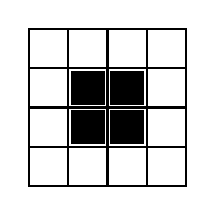
\begin{tikzpicture}[conway]
      \conwaygrid{4}{4};
      \node[cell] at (2,2){}; 
      \node[cell] at (2,3){}; 
      \node[cell] at (3,2){};
      \node[cell] at (3,3){};
    \end{tikzpicture}
    \captionof{figure}{Block}
    \label{fig:block}
  \end{minipage}
  \hspace{.01\textwidth}
  \begin{minipage}{.55\textwidth}
    \centering
    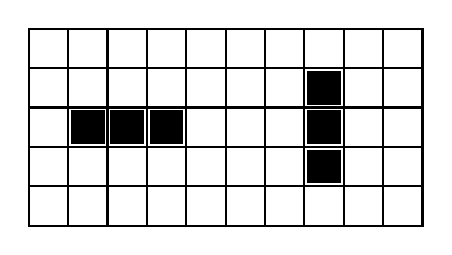
\begin{tikzpicture}[conway]
      \conwaygrid{10}{5};
      \node[cell] at (2,3){}; 
      \node[cell] at (3,3){}; 
      \node[cell] at (4,3){};
      \node[cell] at (8,2){};
      \node[cell] at (8,3){};
      \node[cell] at (8,4){};
    \end{tikzpicture}
    \captionof{figure}{Blinker}
    \label{fig:blinker}
  \end{minipage}
\end{figure}

\begin{figure}
  \begin{minipage}{.45\textwidth}
    \centering
    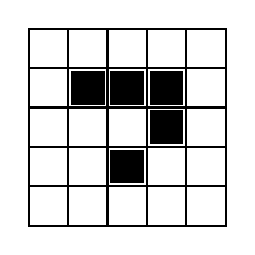
\begin{tikzpicture}[conway]
      \conwaygrid{5}{5};
      \node[cell] at (2,4){}; 
      \node[cell] at (3,4){}; 
      \node[cell] at (4,4){};
      \node[cell] at (4,3){};
      \node[cell] at (3,2){};
    \end{tikzpicture}
    \captionof{figure}{Glider}
    \label{fig:glider}
  \end{minipage}
  \hspace{.01\textwidth}
  \begin{minipage}{.45\textwidth}
    \centering
    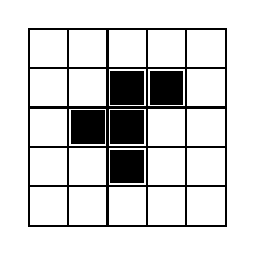
\begin{tikzpicture}[conway]
      \conwaygrid{5}{5};
      \node[cell] at (2,3){}; 
      \node[cell] at (3,2){}; 
      \node[cell] at (3,3){};
      \node[cell] at (3,4){};
      \node[cell] at (4,4){};
    \end{tikzpicture}
    \captionof{figure}{R-pentomino}
    \label{fig:r-pentomino}
  \end{minipage}
\end{figure}

Physicists, biologists, economists, mathematicians, philosophers, generative scientists and others are interested in Conway’s Game of Life in order to observe the way that complex patterns can emerge from the implementation of very simple rules.

Elementary one dimensional version of Game of Life known as Rule 110 is also capable of universal computation \cite{Cook04LifeOneDimensionalUniversal}. It is arguably the simplest known Turing complete system.

% subsection cellular_automaton (end)

\subsection{Swarm Intelligence} % (fold)
\label{sub:swarm_intelligence}

Swarm intelligence \index{Swarm intelligence} systems conists of a population of simple agents, which are following simple rules. They coordinate in decentralized manner and self-organize to achieve a common goal. The swarm intelligence focuses on the collective behaviors that result from the local interactions of the individuals with each other and with their environment. Examples of such systems are colonies of ants and termites, schools of fish, flocks of birds, herds of land animals and bees.

The solutions designed by nature can often be used in other real-world problems.

\subsubsection{Ant colony optimization} % (fold)
\label{ssub:ant_colony_optimization}

Ant colony optimization \index{Ant colony optimization} introduced by Dorigo \cite{Dorigo96Ants} is a class of optimization algorithms for finding better paths through graphs. Ants wander randomly to find some food and return to their colony while laying down pheromone trails. If other ants find such a path, they are likely not to keep travelling at random, but instead to follow the trail, returning and reinforcing it if they eventually find food. Over time, however, the pheromone trail starts to evaporate, thus reducing its attractive strength. The more time it takes for an ant to travel down the path and back again, the more time the pheromones have to evaporate. A short path, by comparison, gets marched over more frequently, and thus the pheromone density becomes higher on shorter paths than longer ones. Pheromone evaporation also has the advantage of avoiding the convergence to a locally optimal solution. If there were no evaporation at all, the paths chosen by the first ants would tend to be excessively attractive to the following ones. In that case, the exploration of the solution space would be constrained. The influence of pheromone evaporation in real ant systems is unclear, but it is very important in artificial systems \cite{Dorigo04Ants}. It has been used to produce near-optimal solutions to the travelling salesman problem. They have an advantage over simulated annealing and genetic algorithm approaches of similar problems when the graph may change dynamically, the ant colony algorithm can be run continuously and adapt to changes in real time. Among other real-world uses are the vehicle routing problem \cite{Rizzoli07AntsVehicle} and improving the efficiency of an electric motor in dry vacuum cleaner \cite{Korosec09AntsVacuum}.

% subsubsection ant_colony_optimization (end)

\subsubsection{Bird flocking} % (fold)
\label{ssub:bird_flocking}

In the natural world, organisms exhibit certain behaviors when traveling in groups. This phenomenon, also known as flocking\index{flocking}, occurs at both microscopic scales (bacteria) and macroscopic scales (birds, fish, insects). Using computers, these patterns can be simulated by creating simple rules for interaction with neighbors and combining them to a complex collective behavior:
\begin{itemize}
  \item Alignment is a behavior that causes a particular agent to line up with agents close by.
  \item Cohesion is a behavior that causes agents to steer towards the center of mass of neighbors - that is, the average position of the agents within a certain radius.
  \item Separation is the behavior that causes an agent to steer away from all of its neighbors to avoid clashes.
\end{itemize}
Reynolds in 1987 first used such rules in a simulation \cite{Reynolds87Flocks}.
Solutions to several problems in other fields have been inspired by flocking. It has been applied to the problem of managing the flight of a number of autonomous unmanned air vehicles \cite{Crowther03FlockingAirVehicles}. They also took into account aerodynamic features of the flock. Another usages are in films to generate crowds which move more realistically, or spatial representation of time-varying information \cite{Moere04FlockingVisual}.

% subsubsection bird_flocking (end)

\subsubsection{Artificial bee colony} % (fold)
\label{ssub:artificial_bee_colony}

Artificial Bee Colony Algorithm is one of the most recent algorithms in the domain of the collective intelligence. It was created by Dervis Karaboga in 2005, who was motivated by the intelligent behavior observed in the domestic bees to take the process of foraging \cite{Karaboga07Bees}. Although, the performance of different optimization algorithm is dependent on applications, some recent works demonstrate that the artificial bee colony is more rapid than either genetic algorithm or particle swarm optimization solving certain problems, especially those with a lot of variables (high-dimensional problems), e.g. protein folding \cite{Li14BeesProtein} and magnetic resonance brain image classification \cite{Zhang11BeesMagnetic}.

% subsubsection artificial_bee_colony (end)

% subsection swarm_intelligence (end)

% Membranes

\subsection{Membrane systems} % (fold)
\label{sub:membrane_systems}

Nature computes not only at the neural or genetic level, but also at the cellular level. In general, any non-trivial biological system has a hierarchical structure where objects and information flows between regions, what can be interpreted as a computation process.

The regions are typically delimited by various types of membranes at different levels from \index{Membrane} cell membranes, through skin membrane to virtual membranes which delimits different parts of an ecosystem.
This hierarchical system can be seen in other field such as distributed computing, where again well delimited computing units coexist and are hierarchically arranged in complex systems from single processors to the internet.

Membranes keep together certain chemicals or information and selectively determines which of them may pass through.

% The notion of membrane structure

From these observations, P\u{a}un \cite{Paun98} introduces the notion of a \index{Membrane!structure} membrane structure as a mathematical representation of hierarchical architectures composed of membranes. It is usually represented as a Venn diagram with all the considered sets being subsets of a unique set and not allowed to be intersected. Every two sets are either one the subset of the other, or disjoint. Outermost membrane (also called skin membrane) delimits the finite ``inside'' and the infinite ``outside''.

Hierarchical structures are usually represented by trees, but membrane structures are visually better viewed as Venn diagram as seen in the figure \ref{fig:membrane_structure}.

\begin{figure}
  \centering
  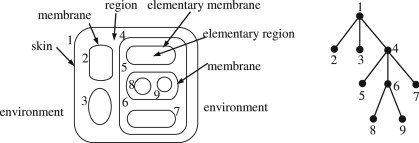
\includegraphics{img/membrane_structure.jpg}
  \caption{The membrane structure of a P system and its associated tree \cite{Zhang20101997AnalyzingRadarSignalsWithMembrane}}
  \label{fig:membrane_structure}
\end{figure}

% Membrane models

Recently, several computational models based on the membrane structure have been created.



% P systems

\subsubsection{P systems} % (fold)
\label{subs:p_systems}

\index{P systems} P systems (see \cite{Paun98}) were introduced in 1998 as a system with membrane structure that contains multisets of objects and rewriting rules that are executed in a maximally parallel manner. Since then, a huge amount of variants have been created with various computation powers. We have investigated the computational power and other attributes of several such variants. Additionally, we propose a new variants various notions of emptyness detection, where the rules can describe what will happen to an object that arrives to an empty membrane.

P systems with existing and newly proposed variants will be discussed in the chapter \ref{cha:p_systems}.

Aside from P systems, other models based on the membrane structure have been created such as the Calculus of Looping Sequences (CLS), which was inspired by P systems.

% subsubsection p_systems (end)


% CLS

\subsubsection{The Calculus of Looping Sequences} % (fold)
\label{subs:calculus_of_looping_sequences}

In the last few years many formalisms originally developed by computer scientists to model systems of interacting components have been applied to biology. Here, we can mention Petri nets (see section \ref{sec:petri_nets}). Others, such as P systems (see chapter \ref{cha:p_systems}), have been proposed as biologically inspired computational models and have been later applied to the description of biological systems.

Many of these models either offer only very low-level interaction primitives or they are specialized to the description of some particular kinds of phenomena such as membrane interactions or protein interactions making the model be not so flexible to allow describing easily new activities observed on membranes without extending the formalism to model such activities.

Barbuti in \cite{Barbuti07CLS} concluded that there is a need for a formalism having a simple notation, having the ability of describing biological systems at different levels of abstractions, having some notions of compositionality and being flexible enough to allow describing new kinds of phenomena as they are discovered, without being specialized to the description of a particular class of systems. The \index{Calculus of Looping Sequences} Calculus of Looping Sequences (CLS) was introduced in \cite{Barbuti07CLS}.

A CLS model consists of a term and a set of rewriting rules. The term is intended to represent the structure of the modeled system and the rewriting rules to represent the events that may cause the system to evolve.

The membrane structure in CLS is defined recursively, consisting of terms and sequences.

We start with defining the syntax of terms. We assume a possibly infinite alphabet $\Sigma$ of symbols.

\begin{definition}
  Terms $T$ and sequences $S$ of CLS are given by the following grammar:
  \begin{align*}
    T ::= S \bigpipe (S)^L\rfloor T \bigpipe T|T\\
    S ::= \eps \bigpipe a \bigpipe S\cdot S
  \end{align*}
  where $a\in \Sigma$ and $\eps$ represents the empty sequence. We denote with $\mathcal T$ the infinite set of terms and with $\mathcal S$ the infinite set of sequences.
\end{definition}

\begin{figure}
  \centering
  \begin{tikzpicture}[node distance=16mm,-triangle 45]
    \node(a){a};
    \node[right=12mm of a](f){f};
    \node[right= of f](g){g};
    \node[right=12mm of g](c){c};
    \node[below=10mm of f](d){d};
    \node[right= of d](e){e};
    \node[below right=16mm and 8mm of d.center](b){b};
    \node[below=10mm of b](description){A representation of the term $(a\cdot b\cdot c)^L\rfloor ((d\cdot e)^L | f\cdot g)$.};
    \draw (a) edge[bend right=60] (b);
    \draw (b) edge[bend right=60] (c);
    \draw (c) edge[bend right=60] (a);
    \draw (d) edge[bend right=60] (e);
    \draw (e) edge[bend right=60] (d);
    \draw (f) edge (g);
  \end{tikzpicture}
  \caption{Example CLS}
  \label{fig:example cls}
\end{figure}

In CLS we have a sequencing operator $\_\cdot\_$, a looping operator $(\_)^L$, a parallel composition operator $\_|\_$ and a containment operator $\_\rfloor\_$. Sequencing can be used to concatenate elements of the alphabet $\Sigma$. The empty sequence $\eps$ denotes the concatenation of zero symbols. A term can be either a sequence or a looping sequence (that is the application of the looping operator to a sequence) containing another term, or the parallel composition of two terms. By definition, looping and containment are always applied together, hence we can consider them as a single binary operator $(\_)^L\rfloor\_$ which applies to one sequence and one term.

\begin{example}
  In the Figure \ref{fig:example cls} we show an example of CLS and its visual representation. The same structure may be represented by syntactically different terms, e.g. $(b\cdot c\cdot a)^L\rfloor (f\cdot g | (e\cdot d)^L)$. We introduce a structural congruence relation to identify such terms.
\end{example}

\begin{definition}
  The structural congruence relations $\equiv_S$ and $\equiv_T$ are the least congruence relations on sequences and on terms, respectively, satisfying the following rules:
  \begin{itemize}
    \item $S_1\cdot(S_2\cdot S_3)\equiv_S (S_1\cdot S_2)\cdot S_3$
    \item $S\cdot\eps\equiv_S \eps\cdot S\equiv_S S$
    \item $S_1\equiv_S S_2$ implies $S_1\equiv_T S_2$ and $(S_1)^L\rfloor T\equiv_T (S_2)^L\rfloor T$
    \item $T_1|T_2\equiv_T T_2|T_1$
    \item $T_1|(T_2|T_3)\equiv_T (T_1|T_2)|T_3$
    \item $T|\eps\equiv_T T$
    \item $(\eps)^L\rfloor\eps\equiv_T\eps$
    \item $(S_1\cdot S_2)^L\rfloor T\equiv_T (S_2\cdot S_1)^L\rfloor T$
  \end{itemize}
\end{definition}

Note that the last rule does not introduce the commutativity of sequences, but only says that looping sequences can rotate.

What could look strange in CLS is the use of looping sequences for the description of membranes, as sequencing is not a commutative operation and this does not correspond to the usual fluid representation of membrane surface in which objects can move freely. What one would expect is to have a multiset or a parallel composition of objects on a membrane. For this reason, a variant called CLS+ was introduced in \cite{Milazzo07CLS}, in which the looping operator can be applied
to a parallel composition of sequences.

\begin{definition}
  Terms $T$, branes $B$ and sequences $S$ of CLS+ are given by the following grammar:
  \begin{align*}
    T ::= S \bigpipe (B)^L\rfloor T \bigpipe T|T\\
    B ::= S \bigpipe B|B\\
    S ::= \eps \bigpipe a \bigpipe S\cdot S
  \end{align*}
\end{definition}

The structural congruence relation of CLS+ is a trivial extension of the one of CLS. The only difference is that commutativity of branes replaces rotation of looping sequences. CLS+ models can be translated into CLS models, while preserving the semantics of the model \cite{Barbuti07CLS}. Milazzo in his PhD thesis \cite{Milazzo07CLS} includes also a simulation of a P system using CLS. The major difficulty was the simulation of the maximal parallel rule application.

% subsubsection calculus_of_looping_sequences (end)

% subsection membrane_systems (end)

% section biologically_inspired_computing_models (end)